%%%% CS 383 HW #3 - hw3-team3.tex
%%%% Due on BBLearn before 10pm on Friday 2/19/2016

\documentclass[11pt]{report}

\usepackage{graphicx}
\usepackage{caption}

\marginparwidth 0.5in 
\oddsidemargin 0.25in 
\evensidemargin 0.25in 
\marginparsep 0.25in
\topmargin 0.0in 
\textwidth 6in \textheight 8.5in

\title{Squire: A Collaborative Software Development Tool}
\author{jank6275, mora5651, boss2849, bolt1003, gall7417, brec9824, snev7821, mars2681}

\begin{document}

\maketitle

\tableofcontents

\chapter{Introduction}

\section{Program Premise}
    \begin{minipage}{1\textwidth}
        \begin{center}
            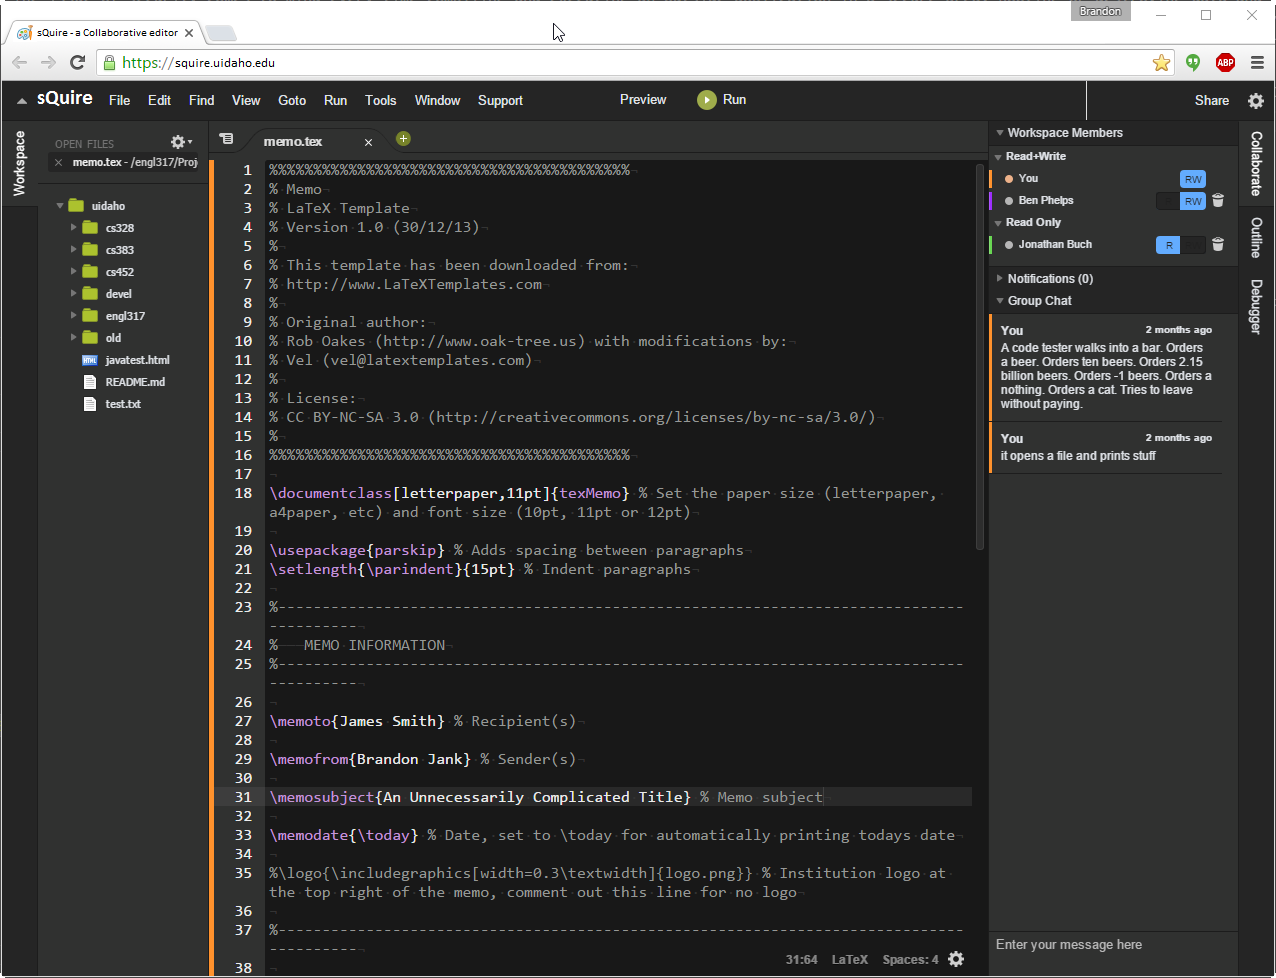
\includegraphics[width=0.7\textwidth]{squire}
        \end{center}
        \captionof{figure}{"Squire is a web-based collaborative software development environment with a project development center. Squire will allow multiple users to edit files and communicate in real time. Projects can be ``stubbed'' out by a user and then other users can join and/or vote to support for their favorite projects. After a certain amount of support, planning, and documentation is reached for a project, the project becomes a fully fleged project and then community development can start. Think ``kickstarter for code'' where people pledge their help with the project and not just financial support."}
    \end{minipage}


\chapter{Class Diagrams}
\section{Overview (brec9824, jank6275)}
    \begin{minipage}{1\textwidth}
        \begin{center}
            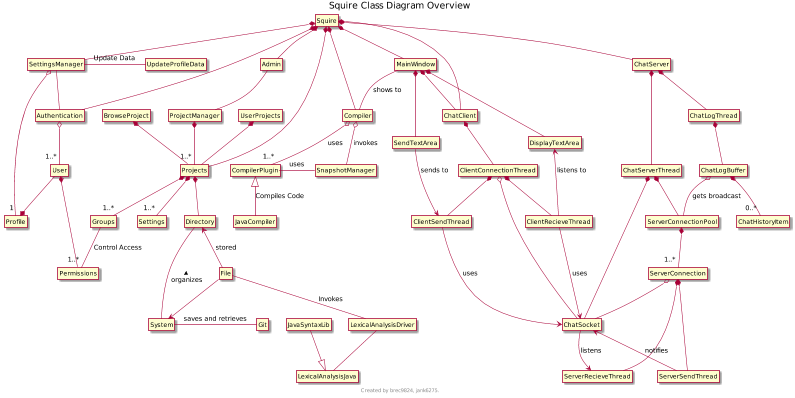
\includegraphics[width=1\textwidth]{diagrams/overview}
        \end{center}
        \captionof{figure}{Class overview of Squire displaying the connections between each subsystem and their classes.}
        %\captionof{figure}{Each team should assign one additional "overview" subteam to draw one or more higher-level overview class diagrams showing the aggregated big picture, with more classes and associations showing but less class detail. This could be one giant diagram, or separate diagrams for inheritance, aggregation, and user-defined associations, or provide an overview along some other structured lines.}
    \end{minipage}


\section{Authentication (mora5651)}
    \begin{minipage}{1\textwidth}
        \begin{center}
            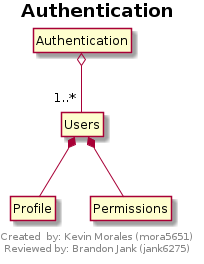
\includegraphics{diagrams/Authentication}
        \end{center}
        \captionof{figure}{Authentication is a security precaution in sQuire that allows the system to verify a user. The authentication process will implement the traditional user/password.}
    \end{minipage}


\section{Project Management (bolt1003)}
    \begin{minipage}{1\textwidth}
        \begin{center}
            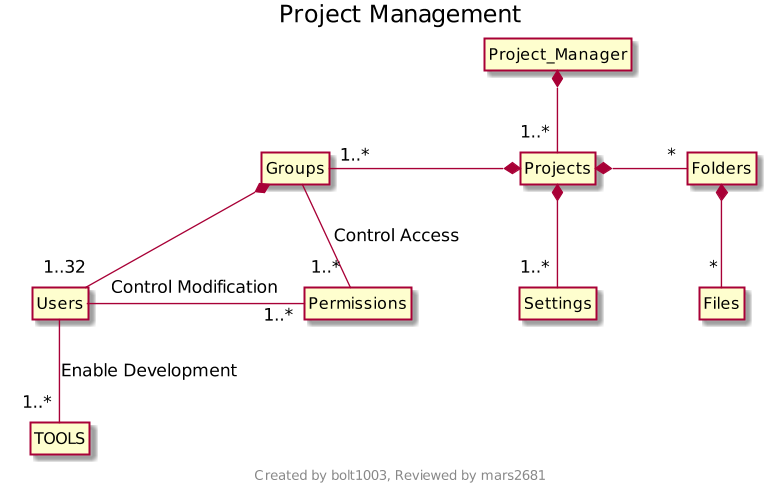
\includegraphics[width=0.9\textwidth]{diagrams/project-management-bolt1003}
        \end{center}
        \captionof{figure}{Project management allows for the group to delicate permissions and create projects}
    \end{minipage}


\section{Project Ideas (mars2681)}
    \begin{minipage}{1\textwidth}
        \begin{center}
            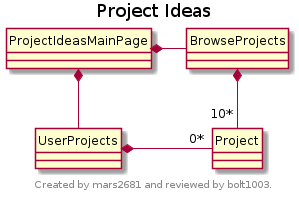
\includegraphics[width=0.7\textwidth]{diagrams/ProjectIdeas-mars2681}
        \end{center}
        \captionof{figure}{The Project Ideas page allows the user to browse other user's projects ideas, as well as create and customize their own project ideas. It starts at the main page. From here, the user can select to view their own projects, and from there create, delete, or edit their ideas. Also at the main page, users can view other projects. Here will be categories of projects, the most popular projects, and new projects. Through browsing these pages, the user can see the description of projects, the amount of support, likes, dislikes, and they can follow and pledge their assistance to the project.}
    \end{minipage}


\section{Settings - Preferences \& Profile (brec9824)}
    \begin{minipage}{1\textwidth}
        \begin{center}
            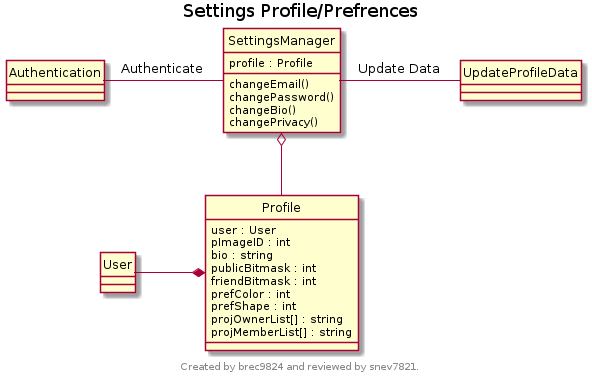
\includegraphics[width=0.9\textwidth]{diagrams/SettingsManager-brec9824}
        \end{center}
        \captionof{figure}{Settings Profile/Prefrences allows for profile viewing and management while maintaining speed with the use of push updates. SettingsManager uses Authentication to verify valid input and to authentic the users data. While SettingsManager uses UpdateUserProfile to push the users data that needs to updated to the server.}
    \end{minipage}


\section{Compiler (boss2849)}
    \begin{minipage}{1\textwidth}
        \begin{center}
            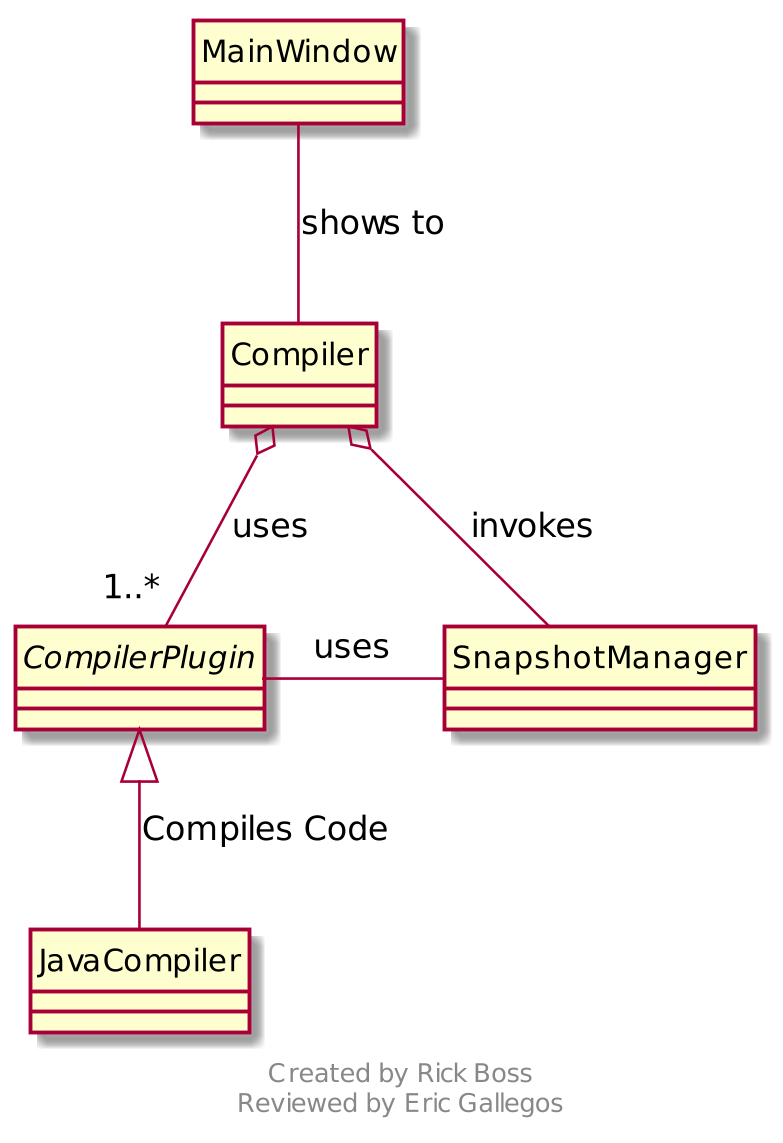
\includegraphics[width=0.7\textwidth]{diagrams/compiler-boss2849}
        \end{center}
        \captionof{figure}{The Compiler is invoked from the main window. From here, the Compiler will select the appropriate CompilerPlugin determined by the configured compiler for the project. The compiler also invokes the SnapshotManager, which stores the current state of the code to be used during compilation. In this simple example, only a JavaCompiler plugin is present, but there can be more than one plugins available in the future. The JavaCompiler plugin retrieves the code snapshot from the SnapshotManager and compiles the code.}
    \end{minipage}


\section{Lexer (gall7417)}
    \begin{minipage}{1\textwidth}
        \begin{center}
            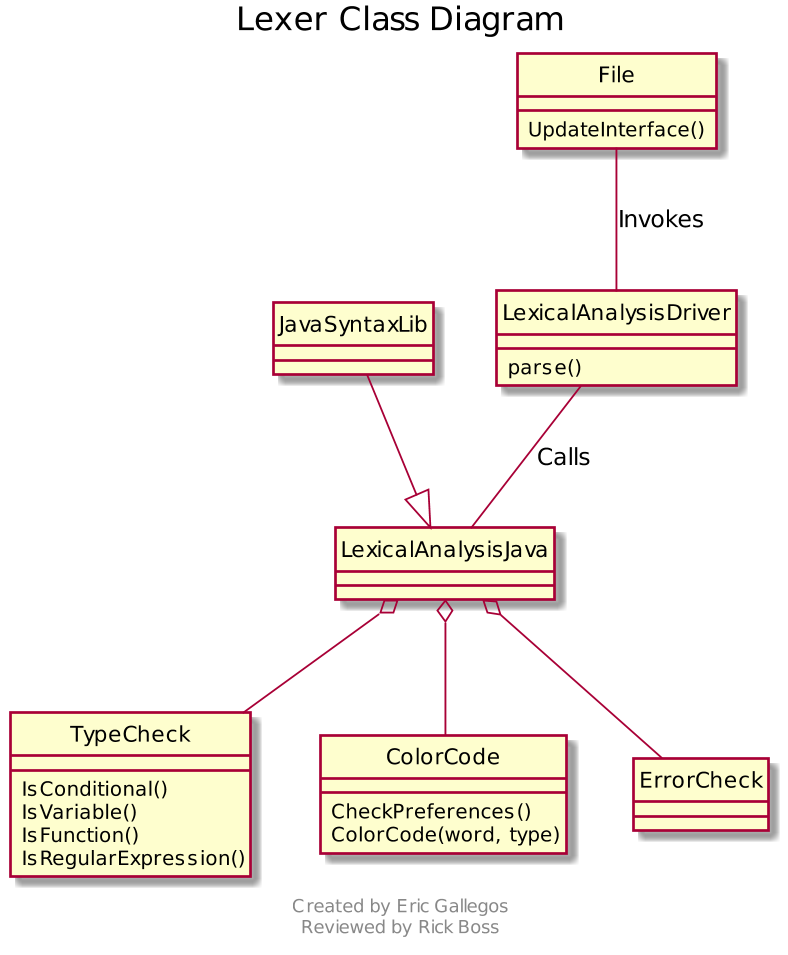
\includegraphics[width=0.9\textwidth]{diagrams/Lexer-gall7417}
        \end{center}
        \captionof{figure}{The File class regularly invokes the Lexical Analysis class to give feedback to users code input. The Lexical Analysis driver calls the corresponding Lexical Analysis class for the language used (Java). This language specific class checks for errors using the ErrorCheck class, searches for word types using the TypeCheck class, and will assign the various words colors to reflect the word types using the ColorCode class.}
    \end{minipage}


\section{Communication (jank6275)}
    \begin{minipage}{1\textwidth}
        \begin{center}
            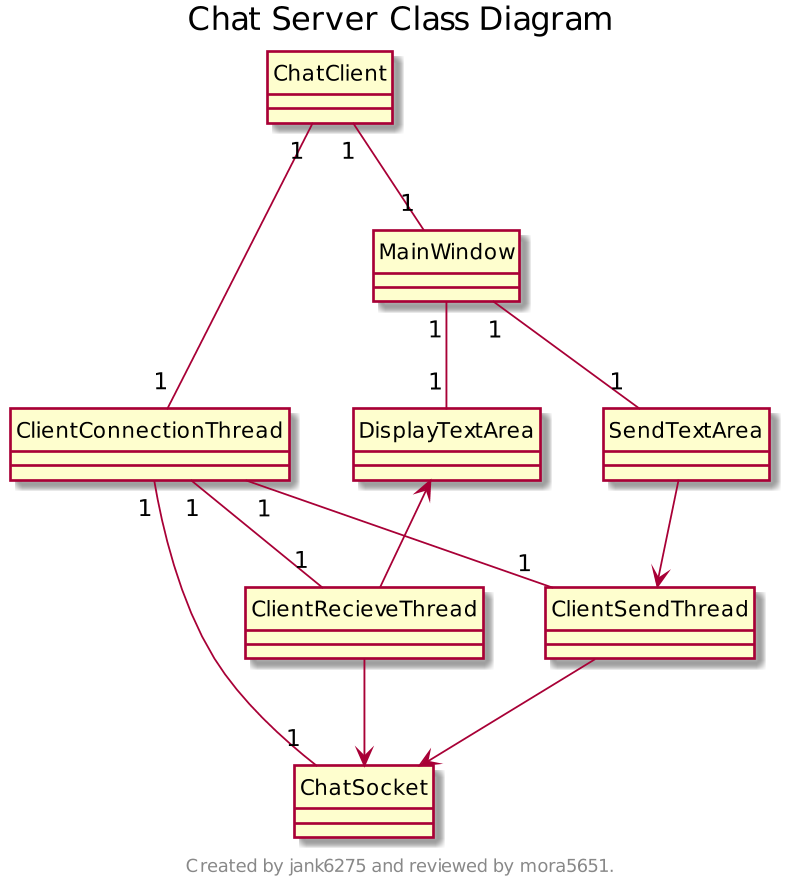
\includegraphics[width=0.7\textwidth]{diagrams/communication-client-jank6275}
        \end{center}
        \captionof{figure}{The ChatClient class will handle text communication in conjuction with the ChatServer class. The Main Window will be home to the ChatClient. The ChatClinet will consist of client send/recieve threads to handle user input/output in the Main Window via the ChatSocket.}
    \end{minipage}
    \begin{minipage}{1\textwidth}
        \begin{center}
            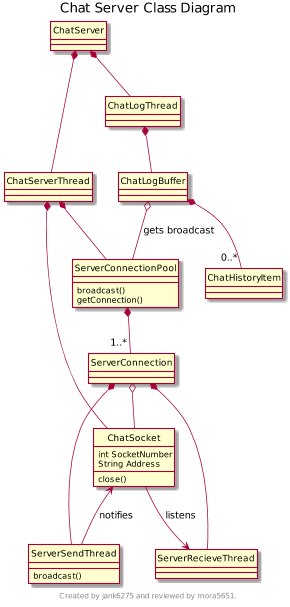
\includegraphics[width=0.5\textwidth]{diagrams/communication-server-jank6275}
        \end{center}
        \captionof{figure}{The ChatServer class will handle text communication between ChatClient(s). The ChatLogThead records any messages broadcast by chat clients in the ServerConnectionPool as a ChatHistoryItem. Each ServerConnection consists of a send and recieve thread that utilize the ChatSocket to broadcast messages.}
    \end{minipage}


\section{Project File Editor (snev7821)}
    \begin{minipage}{1\textwidth}
        \begin{center}
            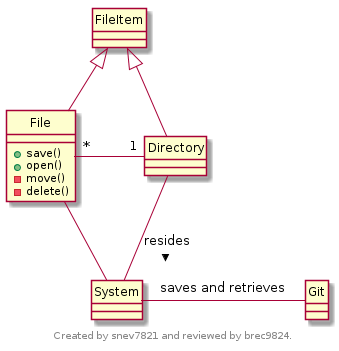
\includegraphics[width=0.7\textwidth]{diagrams/ProjectFileEditor-snev7821}
        \end{center}
        \captionof{figure}{The project File Editor is simply the file system for Squire. It provides basic read/write permission for any user related to a project. Only admins of a project may move project files, delete old files, and create new files.}
    \end{minipage}
    %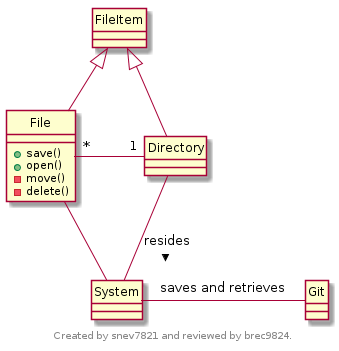
\includegraphics[scale=0.7]{diagrams/ProjectFileEditor-snev7821}
    %The project File Editor is simply the file system for Squire. It provides basic read/write permission for any user related to a project. Only admins of a project may move %project files, delete old files, and create new files.

\end{document}